% This file was converted to LaTeX by Writer2LaTeX ver. 1.0.2
% see http://writer2latex.sourceforge.net for more info
\documentclass[12pt]{article} %scrartcl


% bibliographie
\usepackage[round, authoryear]{natbib}

%accents, language français
\usepackage[utf8]{inputenc}
\usepackage[T1]{fontenc}
\usepackage[english]{babel} %
\usepackage{csquotes}
%\usepackage{xltxtra}

%Lien
\usepackage[colorlinks=true,urlcolor=blue, citecolor=black]{hyperref}

%Image
\usepackage[pdftex]{graphicx}
\usepackage{subcaption}
\usepackage{tikz}
\usetikzlibrary{arrows,shapes}
\newcommand{\HRule}{\rule{\linewidth}{0.5mm}} %Pour la page de titre
\graphicspath{{/home/alain.danet/Dropbox/Shared_TheseAlain/Figures/}}

% Font

% Outline numbering
\setcounter{secnumdepth}{0}
% Set interligne
\linespread{1.5}
% Page layout (geometry)
\usepackage[a4paper]{geometry}
\geometry{left=2.4cm,right=2cm,top=2cm,bottom=2cm}
% Pages styles
\pagestyle{plain}


\begin{document}



\section{Introduction}

Positive interactions between plants have been studied a lot since the very influential paper of \citep{Bertness1994}, followed-up by \citep{Bruno2003}. Results showed positive interactions between pair of plants become often dominant when the environment is harsh for survival of saplings, but result only in a reduction of competition for growth and reproduction\citep{He2013}. Those studies was successful to provide a signal of positive interaction commonness between species pairs. However, no one provide insights from facilitation at community level with a functional approach. One cans imagine when a seed pool arrive in a site, some will germinate (of several species) and several saplings of different species experiment competition between them. Only few of these saplings will become an adult. Previous experiments suggest only one seed by site can germinate. We want here investigate the modulation of interaction between saplings and nurse at community level along a stress gradient.

As \citet{Butterfield2013} suggested, take a functional approach of facilitation will permit us to better understand the context dependence of facilitation. Several studies used Grime's functional types to explain post-hoc general patterns of interaction outcome \citep{Maestre2009,Butterfield2013}. Here, we propose to take a comparative approach of species at community level.

We want to see how interactions are modulated by community composition along a water stress gradient and understand the underlying mechanisms.

\begin{figure}
\begin{center}
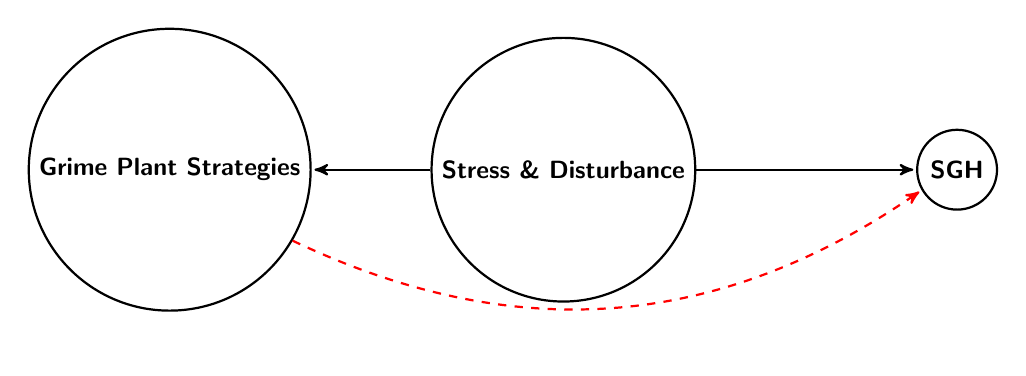
\begin{tikzpicture}[->,>=stealth',shorten >=1pt,auto,node distance=5cm,
                    thick,main node/.style={circle,draw,font=\sffamily\small\bfseries}]

  \node[main node] (1)  {Stress \& Disturbance};
  \node[main node] (2) [right of=1] { SGH };
  \node[main node] (3) [left of=1] {Grime Plant Strategies};

  \path[every node/.style={font=\sffamily\small}]
    (1) edge  node[right] {} (2)
    (1) edge  node {} (3)
    (3) edge [bend right,red, dashed] node  {} (2);
\end{tikzpicture}
\end{center}
\caption{In black: existing links in litterature. In red: Target link to add.}
\end{figure}


\begin{figure}
\begin{center}
\includegraphics[width=0.5\textwidth]{grime_english.pdf}
\end{center}
\caption{Diagram of Grime plant strategies along a gradient of Stress and disturbance.\label{Grime}}
\end{figure}





\section{Methods}

\subsection{Site}

The experiment will take in Alicante (South-East of Spain). Mart's field sites are free to use and those sites seem perfect.

\subsection{Plants}

Plant species were choosen based on spain reviews \citep{McCluney2012,Navarro2006, Jauffret2003}. According to those studies, we classified species which can be used .



\subsection{Design}

We have 3 plant species. I purposed a set of species to Susana and we have to see which can be used. We have 3 treatments: open/patch, water, monoculture/community and 3 blocks (terraces).

For each terrace, we planted 30 saplings by treatment. Nurse micro-sites were choosen randomly and the corresponding open micro-site have been placed Xm around. Each species have been plant alone and in mix with other species. We performed 3 replicates for single species and the same for mix. So we need $10\times5\times3=150$ saplings of each species.


\begin{figure} %Prédictions
\begin{center}
\includegraphics[width=0.75\textwidth]{Experiment.pdf}
\end{center}
\caption{Choosen treatments. Circle: adults; Square: saplings. Saplings are planted in triangular way and position is random in the triangle. Triangle are choosen to be sure saplings are at the same distance of main stem of the nurse. \label{exp}}
\end{figure}

Table \ref{hyp} shows assumptions about results of winning strategies according to stress or disturbance. In Summary, (i) we can think facilitation modulate Grime's prediction, (ii) we also make hypothesis that different strategies have different potential to be facilited.


\begin{table} % Prédictions grime winning hypothesis
\begin{center}
\begin{tabular}{|l|l|l|l|l|l|}
  \hline
  & Control & Water stress & Low grazing & High grazing  \\
  \hline
  Patch & C & C & C & R \\
  \hline
  Open & C & S & S ou R & R \\
  \hline
\end{tabular} 
\end{center}
\caption{Hypothesis about winning plant strategies according to stress or disturbance.  Strategies: C (Competitive), R (Ruderal), S (Stress-tolerator). \label{hyp}}
\end{table}

\subsection{Measurements}
It would be good to measure height canopy and survival regularly to have dynamics of competition. Finally, the final output of competition would be an idea of seed production. 


\subsection{Timing}
\begin{itemize}

\item End January: Drill hole.
\item February: plant saplings, watering them to prevent transplant mortality.
\item March: .
\item June or july: may be one visit to make sure everything is fine and water plants.
\item October: first measure and after application of grazing and water treatment.
\item March: Second measurement

\end{itemize}

\bibliographystyle{apalike}

\bibliography{/home/alain.danet/Dropbox/Shared_TheseAlain/BibTeX/M2-StageM2,/home/alain.danet/Dropbox/Shared_TheseAlain/BibTeX/Thesis}
%\printbibliography
\end{document}
\documentclass[12pt]{article} %scrartcl

%accents, language français
\usepackage[utf8]{inputenc}
\usepackage[T1]{fontenc}

% Outils graphiques
\usepackage{graphicx}
\usepackage{lscape}

\begin{document}

\begin{landscape}

\begin{center}
%\resizebox{\textwidth}{!} {
%{ \footnotesize % Réduire la taille de la police du tableau
\begin{tabular}{ccccc}
\hline 
Loose & Grazing tolerant & Grazing sensitive & Stress-tolerant & Competitive \\ 
\hline 
Teucrium polium & Fagonia cretica & Phlomis purpurea & \textit{Helianthemum squamatum} & \textit{Stipa tenacissima} \\ 

Koeleria vallesiana & Paronichia sufruticosa & Cistus albidus & \textit{Pistacia lentiscus} & \textit{Ligeum spartum} \\ 

Thymus lacaitae & Thymus & Quercus coccifera  & \textit{Lepidium subulatum} &  \\ 

Herniaria fruticosa & Teucrium & Olea europaea & \textit{Retama sphaerocarpa} &  \\ 

 & Sideritis spp. &  &  &  \\ 

 & A. herba-alba &  &  &  \\ 
\hline
\end{tabular} 
%}
%}
\end{center}
\end{landscape}

\end{document}

